\section{Component Tests}
%========================

\subsection{Guillou Ocean Permittivity}
%--------------------------------------
The Guillou ocean permittivity model is taken from \cite{Guillou_etal_1998} where temperature and salinity dependent polynomimal fits for the conductivity, $\sigma$, the static permittivity, \es, the high frequency permittivity, \einf, and the Debye relaxation time, $\tau$, are used to produce complex permittivity values according to the Debye model. The emissivity model invokes the Guillou permittivity procedures only for frequencies less than 20GHz.

This section details the forward/tangent-linear and tangent-linear/adjoint tests performed on the Guillou ocean permittivity procedures. The number and range of input quantities used in the tests are shown in table \ref{tab:guillou_input_range}. A selection of computed forward model Guillou permittivities at different frequencies are shown in figure \ref{fig:guillou_permittivity}. 

\begin{table}[htp]
  \centering
  \begin{tabular}{| c | c | r@{.}l@{ - }r@{.}l | c |}
    \hline
    \textbf{Quantity} & \textbf{\# of Values} & \multicolumn{4}{c|}{\textbf{Range}} & \textbf{Units} \\
    \hline\hline
    Frequency   & 21 &   5&0 &  20&0 & GHz \\
    Salinity    & 21 &  20&0 &  40&0 & \textperthousand \\
    Temperature & 21 & 273&0 & 303&0 & K \\
    \hline
  \end{tabular}
  \caption{Range of test input data to the Guillou ocean permittivity procedures.}
  \label{tab:guillou_input_range}
\end{table}

\begin{figure}[htp]
  \centering
  \begin{tabular}{c c}
    \multicolumn{2}{c}{\sffamily\textbf{5.0GHz}}\\
    \textsf{(a) Real part} &
    \textsf{(b) Imaginary part} \\
    \includegraphics[bb=135 240 508 540,clip,scale=0.5]{graphics/Guillou/e_re_5.00GHz.eps} &
    \includegraphics[bb=135 240 508 540,clip,scale=0.5]{graphics/Guillou/e_im_5.00GHz.eps} \\\\

    \multicolumn{2}{c}{\sffamily\textbf{10.25GHz}}\\
    \textsf{(c) Real part} &
    \textsf{(d) Imaginary part} \\
    \includegraphics[bb=135 240 508 540,clip,scale=0.5]{graphics/Guillou/e_re_10.25GHz.eps} &
    \includegraphics[bb=135 240 508 540,clip,scale=0.5]{graphics/Guillou/e_im_10.25GHz.eps} \\\\

    \multicolumn{2}{c}{\sffamily\textbf{20.0GHz}}\\
    \textsf{(e) Real part} &
    \textsf{(f) Imaginary part} \\
    \includegraphics[bb=135 240 508 540,clip,scale=0.5]{graphics/Guillou/e_re_20.00GHz.eps} &
    \includegraphics[bb=135 240 508 540,clip,scale=0.5]{graphics/Guillou/e_im_20.00GHz.eps}
  \end{tabular}
  \caption{Real and imaginary parts of the computed Guillou permittivity as a function of temperature and salinity for three frequencies $\le$ 20GHz}
  \label{fig:guillou_permittivity}
\end{figure}


\subsubsection{FWD/TL Test Results}
%..................................
\label{sec:fwdtl_guillou}
The description of the FWD/TL tests for routines with complex valued output was given in section \ref{sec:fwdtl_test}. Some representative results for the Guillou permittivity routines are shown in figure \ref{fig:fwdtl_a0.1000_guillou} for 7.25GHz and an alpha value of 0.1, and in figure \ref{fig:fwdtl_a0.0001_guillou} for 16.25GHz and an alpha value of 0.0001. The maximum tolerance residual for each value of alpha is shown in table \ref{tab:fwdtl_guillou_alpha}.
\begin{table}[htp]
  \centering
  \begin{tabular}{| c | c |}
    \hline
    \boldmath$\alpha$\unboldmath & \textbf{Tolerance residual,} \boldmath$t_r$\unboldmath \\
    \hline\hline
    0.1    & 6.0e-08 \\
    0.01   & 6.0e-10 \\
    0.001  & 5.0e-11 \\
    0.0001 & 4.0e-10 \\
    \hline
  \end{tabular}
  \caption{Maximum tolerance residuals for the Guillou permittivity FWD/TL tests.}
  \label{tab:fwdtl_guillou_alpha}
\end{table}
As would be expected, as alpha decreases so do the tolerance residuals since, for smaller and smaller perturbations the forward model reponse becomes more linear, i.e. the residuals are more due to noise than non-linearity. This is quite evident when one compares the residual surfaces of figure \ref{fig:fwdtl_a0.1000_guillou}(e) and (f) with those in figure \ref{fig:fwdtl_a0.0001_guillou}(e) and (f). As the alpha value decreases, the residuals contain less information about the polynomial dependencies of the Guillou permittivity on temperature (higher orders) and salinity (linear). It it surmised that the $O(10^{-10})$ tolerance limit for the FWD/TL tests is due to the propagation of precision errors in the model parameterisation. In any case, the results are well below the precision of the measurements used in generating the fit coefficients as reported in \cite{Guillou_etal_1998}.

\begin{figure}[htp]
  \centering
  \begin{tabular}{c c}
    \multicolumn{2}{c}{\sffamily\textbf{Non-linear difference}}\\
    \textsf{(a)} $\Delta\Re\{\epsilon\}$ &
    \textsf{(b)} $\Delta\Im\{\epsilon\}$ \\
    \hspace{1.0em}\includegraphics[bb=125 240 508 540,clip,scale=0.5]{graphics/Guillou/FWDTL/FWDde_a0.1000_re_7.25GHz.eps} &
    \includegraphics[bb=125 240 508 540,clip,scale=0.5]{graphics/Guillou/FWDTL/FWDde_a0.1000_im_7.25GHz.eps} \\\\
    \multicolumn{2}{c}{\sffamily\textbf{Tangent-linear response}}\\
    \textsf{(c)} $\Re\{\de\}$ &
    \textsf{(d)} $\Im\{\de\}$ \\
    \hspace{1.0em}\includegraphics[bb=125 240 508 540,clip,scale=0.5]{graphics/Guillou/FWDTL/TLde_a0.1000_re_7.25GHz.eps} &
    \includegraphics[bb=125 240 508 540,clip,scale=0.5]{graphics/Guillou/FWDTL/TLde_a0.1000_im_7.25GHz.eps} \\\\
    \multicolumn{2}{c}{\sffamily\textbf{Forward/tangent-linear test result}}\\
    \textsf{(e)} $|\Delta\Re\{\epsilon\} - \Re\{\de\}|$ &
    \textsf{(f)} $|\Delta\Im\{\epsilon\} - \Im\{\de\}|$ \\
    \includegraphics[bb=110 240 508 540,clip,scale=0.5]{graphics/Guillou/FWDTL/FWDTLtest_a0.1000_re_7.25GHz.eps} & 
    \includegraphics[bb=120 240 508 540,clip,scale=0.5]{graphics/Guillou/FWDTL/FWDTLtest_a0.1000_im_7.25GHz.eps}
  \end{tabular}
  \caption{Real and imaginary parts of the computed Guillou complex permittivities at 7.25GHz for the forward/tangent-linear test with $\alpha$=0.1. \textbf{(a)} Real component non-linear difference.  \textbf{(b)} Imaginary component non-linear difference. \textbf{(c)} Real component tangent-linear response. \textbf{(d)} Imaginary component tangent-linear response. \textbf{(e)} Real component test residual. \textbf{(f)} Imaginary component test residual.}
  \label{fig:fwdtl_a0.1000_guillou}
\end{figure}

\begin{figure}[htp]
  \centering
  \begin{tabular}{c c}
    \multicolumn{2}{c}{\sffamily\textbf{Non-linear difference}}\\
    \textsf{(a)} $\Delta\Re\{\epsilon\}$ &
    \textsf{(b)} $\Delta\Im\{\epsilon\}$ \\
    \hspace{1.0em}\includegraphics[bb=127 240 508 540,clip,scale=0.5]{graphics/Guillou/FWDTL/FWDde_a0.0001_re_16.25GHz.eps} &
    \hspace{1.0em}\includegraphics[bb=127 240 508 540,clip,scale=0.5]{graphics/Guillou/FWDTL/FWDde_a0.0001_im_16.25GHz.eps} \\\\
    \multicolumn{2}{c}{\sffamily\textbf{Tangent-linear response}}\\
    \textsf{(c)} $\Re\{\de\}$ &
    \textsf{(d)} $\Im\{\de\}$ \\
    \hspace{1.0em}\includegraphics[bb=127 240 508 540,clip,scale=0.5]{graphics/Guillou/FWDTL/TLde_a0.0001_re_16.25GHz.eps} &
    \hspace{1.0em}\includegraphics[bb=127 240 508 540,clip,scale=0.5]{graphics/Guillou/FWDTL/TLde_a0.0001_im_16.25GHz.eps} \\\\
    \multicolumn{2}{c}{\sffamily\textbf{Forward/tangent-linear test result}}\\
    \textsf{(e)} $|\Delta\Re\{\epsilon\} - \Re\{\de\}|$ &
    \textsf{(f)} $|\Delta\Im\{\epsilon\} - \Im\{\de\}|$ \\
    \includegraphics[bb=115 240 508 540,clip,scale=0.5]{graphics/Guillou/FWDTL/FWDTLtest_a0.0001_re_16.25GHz.eps} & 
    \includegraphics[bb=109 240 508 540,clip,scale=0.5]{graphics/Guillou/FWDTL/FWDTLtest_a0.0001_im_16.25GHz.eps}
  \end{tabular}
  \caption{Real and imaginary parts of the computed Guillou complex permittivities at 16.25GHz for the forward/tangent-linear test with $\alpha$=0.0001. \textbf{(a)} Real component non-linear difference.  \textbf{(b)} Imaginary component non-linear difference. \textbf{(c)} Real component tangent-linear response. \textbf{(d)} Imaginary component tangent-linear response. \textbf{(e)} Real component test residual. \textbf{(f)} Imaginary component test residual.}
  \label{fig:fwdtl_a0.0001_guillou}
\end{figure}


\subsubsection{TL/AD Test Results}
%.................................
\label{sec:tlad_guillou}
Following the description of the TL/AD tests in section \ref{sec:tlad_test} for routines with real valued input and complex valued output, the TL/AD test performed for the Guillou permittivity routines was,
\begin{equation}
  \underbrace{\left[\Re\{\de\}^{2} + \Im\{\de\}^{2}\right]}_{\mathbf{TL}^{T}\mathbf{TL}} - \underbrace{\left[\delta{T}.\dstar {T} + \delta{S}.\dstar {S}\right]}_{\mathbf{\delta x}^{T}\mathbf{AD}(TL)} = 0
  \label{eqn:tlad_guillou}
\end{equation}
where $T$ and $S$ are the sea surface temperature and salinity respectively (TL inputs are set to 0.1 in both cases), and $\epsilon$ is the complex permittivity. Examples of the intermediate and final quantities used in this test are shown in figure \ref{fig:tlad_7.25GHz_guillou} for $f = 7.25$GHz and \ref{fig:tlad_16.25GHz_guillou} for $f = 16.25$GHz. The differences between the values represented in figures \ref{fig:tlad_7.25GHz_guillou}(e) and (f) and \ref{fig:tlad_16.25GHz_guillou}(e) and (f) are shown in figure \ref{fig:tlad_test_guillou}. In both cases, the differences were within numerical precision. These results are typical of the other frequencies tested.

\begin{figure}[htp]
  \centering
  \begin{tabular}{c c}
    \multicolumn{2}{c}{\sffamily\textbf{Tangent-linear permittivity}}\\
    \textsf{(a)} $\Re\{\de\}$ &
    \textsf{(b)} $\Im\{\de\}$ \\
    \includegraphics[bb=125 240 508 540,clip,scale=0.5]{graphics/Guillou/TLAD/e_TL_re_7.25GHz.eps} &
    \includegraphics[bb=125 240 508 540,clip,scale=0.5]{graphics/Guillou/TLAD/e_TL_im_7.25GHz.eps} \\\\
    \multicolumn{2}{c}{\sffamily\textbf{Adjoint temperature and salinity}}\\
    \textsf{(c)} $\dstar {T}$ &
    \textsf{(d)} $\dstar {S}$ \\
    \includegraphics[bb=125 240 508 540,clip,scale=0.5]{graphics/Guillou/TLAD/t_AD_7.25GHz.eps} &
    \includegraphics[bb=120 240 508 540,clip,scale=0.5]{graphics/Guillou/TLAD/s_AD_7.25GHz.eps} \\\\
    \multicolumn{2}{c}{\sffamily\textbf{Test quantities}}\\
    \textsf{(e)} $\mathbf{TL}^{T}\mathbf{TL}$ &
    \textsf{(f)} $\mathbf{\delta x}^{T}\mathbf{AD}(TL)$ \\
    \includegraphics[bb=120 240 508 540,clip,scale=0.5]{graphics/Guillou/TLAD/TLtTL_7.25GHz.eps} & 
    \includegraphics[bb=120 240 508 540,clip,scale=0.5]{graphics/Guillou/TLAD/dxtAD_7.25GHz.eps}
  \end{tabular}
  \caption{Example of quantities used to test the TL/AD Guillou permittivity routines for $\delta{T}$ and $\delta{S}$ inputs of 0.1 at 7.25GHz. \textbf{(a)} Real component of the tangent-linear permittivity.  \textbf{(b)} Imaginary component of the tangent-linear permittivity. \textbf{(c)} Temperature adjoint. \textbf{(d)} Salinity adjoint. \textbf{(e)} Tangent-linear test result (see eqn.\ref{eqn:tlad_guillou}). \textbf{(f)} Adjoint test result (see eqn.\ref{eqn:tlad_guillou}).}
  \label{fig:tlad_7.25GHz_guillou}
\end{figure}

\begin{figure}[htp]
  \centering
  \begin{tabular}{c c}
    \multicolumn{2}{c}{\sffamily\textbf{Tangent-linear permittivity}}\\
    \textsf{(a)} $\Re\{\de\}$ &
    \textsf{(b)} $\Im\{\de\}$ \\
    \includegraphics[bb=130 240 508 540,clip,scale=0.5]{graphics/Guillou/TLAD/e_TL_re_16.25GHz.eps} &
    \includegraphics[bb=125 240 508 540,clip,scale=0.5]{graphics/Guillou/TLAD/e_TL_im_16.25GHz.eps} \\\\
    \multicolumn{2}{c}{\sffamily\textbf{Adjoint temperature and salinity}}\\
    \textsf{(c)} $\dstar {T}$ &
    \textsf{(d)} $\dstar {S}$ \\
    \includegraphics[bb=130 240 508 540,clip,scale=0.5]{graphics/Guillou/TLAD/t_AD_16.25GHz.eps} &
    \includegraphics[bb=120 240 508 540,clip,scale=0.5]{graphics/Guillou/TLAD/s_AD_16.25GHz.eps} \\\\
    \multicolumn{2}{c}{\sffamily\textbf{Test quantities}}\\
    \textsf{(e)} $\mathbf{TL}^{T}\mathbf{TL}$ &
    \textsf{(f)} $\mathbf{\delta x}^{T}\mathbf{AD}(TL)$ \\
    \includegraphics[bb=120 240 508 540,clip,scale=0.5]{graphics/Guillou/TLAD/TLtTL_16.25GHz.eps} & 
    \includegraphics[bb=120 240 508 540,clip,scale=0.5]{graphics/Guillou/TLAD/dxtAD_16.25GHz.eps}
  \end{tabular}
  \caption{Example of quantities used to test the TL/AD Guillou permittivity routines for $\delta{T}$ and $\delta{S}$ inputs of 0.1 at 16.25GHz. \textbf{(a)} Real component of the tangent-linear permittivity.  \textbf{(b)} Imaginary component of the tangent-linear permittivity. \textbf{(c)} Temperature adjoint. \textbf{(d)} Salinity adjoint. \textbf{(e)} Tangent-linear test result (see eqn.\ref{eqn:tlad_guillou}). \textbf{(f)} Adjoint test result (see eqn.\ref{eqn:tlad_guillou}).}
  \label{fig:tlad_16.25GHz_guillou}
\end{figure}

\begin{figure}[htp]
  \centering
  \begin{tabular}{c}
    \textsf{(a) $\mathbf{TL}^{T}\mathbf{TL} - \mathbf{\delta x}^{T}\mathbf{AD}(TL)$ for $f$=7.25GHz}\\
    \includegraphics[bb=115 240 508 525,clip,scale=0.8]{graphics/Guillou/TLAD/TLtTL-dxtAD_7.25GHz.eps}\\\\\\
    \textsf{(b) $\mathbf{TL}^{T}\mathbf{TL} - \mathbf{\delta x}^{T}\mathbf{AD}(TL)$ for $f$=16.25GHz}\\
    \includegraphics[bb=115 240 508 525,clip,scale=0.8]{graphics/Guillou/TLAD/TLtTL-dxtAD_16.25GHz.eps}\\\\
  \end{tabular}
  \caption{Guillou permittivity model TL/AD test results for the two test frequencies indicating TL/AD agreement to numerical precision. \textbf{(a)} Result for 7.25GHz (See figure \ref{fig:tlad_7.25GHz_guillou}). \textbf{(b)} Result for 16.25GHz (See figure \ref{fig:tlad_16.25GHz_guillou}).}
  \label{fig:tlad_test_guillou}
\end{figure}



\subsection{Fresnel Reflectivity}
%--------------------------------
The derivations of the Fresnel reflectivity equations used in the model are given in appendix \ref{sec:fresnel_equations}. This section details the forward/tangent-linear and tangent-linear/adjoint tests performed on the Fresnel reflectivity procedures. The number and range of input quantities used in the tests are shown in table \ref{tab:fresnel_input_range}. A selection of computed forward model reflectivities at different incidence angles are shown in figure \ref{fig:fresnel_reflectivity}.
\begin{table}[htp]
  \centering
  \begin{tabular}{| c | c | r@{.}l@{ - }r@{.}l | c |}
    \hline
    \textbf{Quantity} & \textbf{\# of Values} & \multicolumn{4}{c|}{\textbf{Range}} & \textbf{Units} \\
    \hline\hline
    Angle, $\theta_i$ &  7 &  0&0 &  60&0 & degrees \\
    $\Re\{\epsilon\}$ & 21 &  5&0 &  75&0 & F.m$^{-1}$ (?) \\
    $\Im\{\epsilon\}$ & 21 & -5&0 & -31&0 & F.m$^{-1}$ (?) \\
    \hline
  \end{tabular}
  \caption{Range of test input data to the Fresnel reflectivity procedures.}
  \label{tab:fresnel_input_range}
\end{table}

\begin{figure}[htp]
  \centering
  \begin{tabular}{c c}
    \multicolumn{2}{c}{\boldmath$\theta_i$\unboldmath\sffamily\textbf{=0.0}\boldmath$^\circ$\unboldmath}\\
    \textsf{(a) Vertical} &
    \textsf{(b) Horizontal} \\
    \includegraphics[bb=135 240 508 540,clip,scale=0.5]{graphics/Fresnel/rv_z0.0.eps} &
    \includegraphics[bb=135 240 508 540,clip,scale=0.5]{graphics/Fresnel/rh_z0.0.eps} \\\\

    \multicolumn{2}{c}{\boldmath$\theta_i$\unboldmath\sffamily\textbf{=30.0}\boldmath$^\circ$\unboldmath}\\
    \textsf{(c) Vertical} &
    \textsf{(d) Horizontal} \\
    \includegraphics[bb=135 240 508 540,clip,scale=0.5]{graphics/Fresnel/rv_z30.0.eps} &
    \includegraphics[bb=135 240 508 540,clip,scale=0.5]{graphics/Fresnel/rh_z30.0.eps} \\\\

    \multicolumn{2}{c}{\boldmath$\theta_i$\unboldmath\sffamily\textbf{=60.0}\boldmath$^\circ$\unboldmath}\\
    \textsf{(e) Vertical} &
    \textsf{(f) Horizontal} \\
    \includegraphics[bb=135 240 508 540,clip,scale=0.5]{graphics/Fresnel/rv_z60.0.eps} &
    \includegraphics[bb=135 240 508 540,clip,scale=0.5]{graphics/Fresnel/rh_z60.0.eps}
  \end{tabular}
  \caption{Vertical and horizontal Fresnel reflectivities as a function of the real and imaginary part of the permittivity for three incidence angles.}
  \label{fig:fresnel_reflectivity}
\end{figure}


\subsubsection{FWD/TL Test Results}
%..................................
The description of the FWD/TL tests for routines with reall valued output was given in section \ref{sec:fwdtl_test}. Some representative results for the Fresnel reflectivity FWD/TL tests are shown in figure \ref{fig:fwdtl_a0.1000_fresnel} for an incidence angle of $20^{\circ}$ and an alpha value of 0.1 and in figure \ref{fig:fwdtl_a0.0001_fresnel} for an incidence angle of $40^{\circ}$ and an alpha value of 0.0001. The maximum tolerance residual for each value of alpha is shown in table \ref{tab:fwdtl_fresnel_alpha}.
\begin{table}[htp]
  \centering
  \begin{tabular}{| c | c |}
    \hline
    \boldmath$\alpha$\unboldmath & \textbf{Tolerance residual,} \boldmath$t_r$\unboldmath \\
    \hline\hline
    0.1    & 7.0e-09 \\
    0.01   & 7.0e-11 \\
    0.001  & 7.0e-13 \\
    0.0001 & 3.0e-12 \\
    \hline
  \end{tabular}
  \caption{Maximum tolerance residuals for the Fresnel reflectivity FWD/TL tests.}
  \label{tab:fwdtl_fresnel_alpha}
\end{table}
As with the permittivity FWD/TL test, as the alpha value decreases so does the tolerance residual. Interestingly, the tolerance residual for the smallest alpha value follows the same pattern as for the permittivity in that it is an order of magnitude larger than that for the next larger alpha value case. Additional tests showed that as alpha is decreased even further, the associated tolerance residual steadily increases indicating the results are at the precision limit.

\begin{figure}[htp]
  \centering
  \begin{tabular}{c c}
    \multicolumn{2}{c}{\sffamily\textbf{Non-linear difference}}\\
    \textsf{(a)} $\Delta r_v$ &
    \textsf{(b)} $\Delta r_h$ \\
    \includegraphics[bb=120 240 508 540,clip,scale=0.5]{graphics/Fresnel/FWDTL/FWDdrv_a0.1000_z20.0.eps} &
    \includegraphics[bb=120 240 508 540,clip,scale=0.5]{graphics/Fresnel/FWDTL/FWDdrh_a0.1000_z20.0.eps} \\\\
    \multicolumn{2}{c}{\sffamily\textbf{Tangent-linear response}}\\
    \textsf{(c)} $\delta r_v$ &
    \textsf{(d)} $\delta r_h$ \\
    \includegraphics[bb=120 240 508 540,clip,scale=0.5]{graphics/Fresnel/FWDTL/TLdrv_a0.1000_z20.0.eps} &
    \includegraphics[bb=120 240 508 540,clip,scale=0.5]{graphics/Fresnel/FWDTL/TLdrh_a0.1000_z20.0.eps} \\\\
    \multicolumn{2}{c}{\sffamily\textbf{Forward/tangent-linear test result}}\\
    \textsf{(e)} $|\Delta r_v - \delta r_v|$ &
    \textsf{(f)} $|\Delta r_h - \delta r_h|$ \\
    \includegraphics[bb=120 240 508 540,clip,scale=0.5]{graphics/Fresnel/FWDTL/FWDTLtestrv_a0.1000_z20.0.eps} & 
    \includegraphics[bb=120 240 508 540,clip,scale=0.5]{graphics/Fresnel/FWDTL/FWDTLtestrh_a0.1000_z20.0.eps}
  \end{tabular}
  \caption{Vertical and horizontal Fresnel reflectivities at $\theta_i$=20.0$^\circ$ for the forward/tangent-linear test with $\alpha$=0.1. \textbf{(a)} Vertical component non-linear difference.  \textbf{(b)} Horizontal component non-linear difference. \textbf{(c)} Vertical component tangent-linear response. \textbf{(d)} Horizontal component tangent-linear response. \textbf{(e)} Vertical component test residual. \textbf{(f)} Horizontal component test residual.}
  \label{fig:fwdtl_a0.1000_fresnel}
\end{figure}

\begin{figure}[htp]
  \centering
  \begin{tabular}{c c}
    \multicolumn{2}{c}{\sffamily\textbf{Non-linear difference}}\\
    \textsf{(a)} $\Delta r_v$ &
    \textsf{(b)} $\Delta r_h$ \\
    \includegraphics[bb=115 240 508 540,clip,scale=0.5]{graphics/Fresnel/FWDTL/FWDdrv_a0.0001_z40.0.eps} &
    \includegraphics[bb=120 240 508 540,clip,scale=0.5]{graphics/Fresnel/FWDTL/FWDdrh_a0.0001_z40.0.eps} \\\\
    \multicolumn{2}{c}{\sffamily\textbf{Tangent-linear response}}\\
    \textsf{(c)} $\delta r_v$ &
    \textsf{(d)} $\delta r_h$ \\
    \includegraphics[bb=115 240 508 540,clip,scale=0.5]{graphics/Fresnel/FWDTL/TLdrv_a0.0001_z40.0.eps} &
    \includegraphics[bb=120 240 508 540,clip,scale=0.5]{graphics/Fresnel/FWDTL/TLdrh_a0.0001_z40.0.eps} \\\\
    \multicolumn{2}{c}{\sffamily\textbf{Forward/tangent-linear test result}}\\
    \textsf{(e)} $|\Delta r_v - \delta r_v|$ &
    \textsf{(f)} $|\Delta r_h - \delta r_h|$ \\
    \includegraphics[bb=110 240 508 540,clip,scale=0.5]{graphics/Fresnel/FWDTL/FWDTLtestrv_a0.0001_z40.0.eps} & 
    \includegraphics[bb=110 240 508 540,clip,scale=0.5]{graphics/Fresnel/FWDTL/FWDTLtestrh_a0.0001_z40.0.eps}
  \end{tabular}
  \caption{Vertical and horizontal Fresnel reflectivities at $\theta_i$=40.0$^\circ$ for the forward/tangent-linear test with $\alpha$=0.0001. \textbf{(a)} Vertical component non-linear difference.  \textbf{(b)} Horizontal component non-linear difference. \textbf{(c)} Vertical component tangent-linear response. \textbf{(d)} Horizontal component tangent-linear response. \textbf{(e)} Vertical component test residual. \textbf{(f)} Horizontal component test residual.}
  \label{fig:fwdtl_a0.0001_fresnel}
\end{figure}


\subsubsection{TL/AD Test Results}
%.................................
Following the description of the TL/AD test in section \ref{sec:tlad_test} for routines with complex valued input and real valued output, the TL/AD test performed for the Fresnel reflectivity routines was,
\begin{equation}
  \underbrace{\left[\delta r_{v}^2 + \delta r_{h}^2\right]}_{\mathbf{TL}^{T}\mathbf{TL}} - \underbrace{\left[\Re\{\de\}.\Re\{\dstar \epsilon\} + \Im\{\de\}.\Im\{\dstar \epsilon\}\right]}_{\mathbf{\delta x}^{T}\mathbf{AD}(TL)} = 0
  \label{eqn:tlad_fresnel}
\end{equation}
where $\epsilon$ is the complex permittivity (TL inputs set to 0.1), and $r_v$ and $r_h$ are the vertical and horizontal reflectivities respectively. Examples of the intermediate and final quantities used in this test are shown in figure \ref{fig:tlad_z20.0_fresnel} for $\theta_{i} = 20^{\circ}$, and figure \ref{fig:tlad_z40.0_fresnel} for $\theta_{i} = 40^{\circ}$. The differences between figure \ref{fig:tlad_z20.0_fresnel}(e) and (f), and figure \ref{fig:tlad_z40.0_fresnel}(e) and (f) are shown in figure \ref{fig:tlad_test_fresnel}. In both cases, the differences are within numerical precision. These results are typical of the other incidence angles tested.

\begin{figure}[htp]
  \centering
  \begin{tabular}{c c}
    \multicolumn{2}{c}{\sffamily\textbf{Tangent-linear reflectivites}}\\
    \textsf{(a)} $\delta r_v$ &
    \textsf{(b)} $\delta r_h$ \\
    \includegraphics[bb=120 240 508 540,clip,scale=0.5]{graphics/Fresnel/TLAD/rv_TL_z20.0.eps} &
    \includegraphics[bb=120 240 508 540,clip,scale=0.5]{graphics/Fresnel/TLAD/rv_TL_z20.0.eps} \\\\
    \multicolumn{2}{c}{\sffamily\textbf{Adjoint permittivities}}\\
    \textsf{(c)} $\Re\{\dstar \epsilon\}$ &
    \textsf{(d)} $\Im\{\dstar \epsilon\}$ \\
    \includegraphics[bb=115 240 508 540,clip,scale=0.5]{graphics/Fresnel/TLAD/Re_e_AD_z20.0.eps} &
    \includegraphics[bb=110 240 508 540,clip,scale=0.5]{graphics/Fresnel/TLAD/Im_e_AD_z20.0.eps} \\\\
    \multicolumn{2}{c}{\sffamily\textbf{Test quantities}}\\
    \textsf{(e)} $\mathbf{TL}^{T}\mathbf{TL}$ &
    \textsf{(f)} $\mathbf{\delta x}^{T}\mathbf{AD}(TL)$ \\
    \includegraphics[bb=110 240 508 540,clip,scale=0.5]{graphics/Fresnel/TLAD/TLtTL_z20.0.eps} & 
    \includegraphics[bb=110 240 508 540,clip,scale=0.5]{graphics/Fresnel/TLAD/dxtAD_z20.0.eps}
  \end{tabular}
  \caption{Example of quantities used to test the TL/AD Fresnel reflectivity routines for $\Re\{\de\}$ and $\Im\{\de\}$ inputs of 0.1 at an incidence angle of 20$^{\circ}$. \textbf{(a)} Tangent-linear vertical reflectivity. \textbf{(b)} Tangent-linear horizontal reflectivity. \textbf{(c)} Real component of the adjoint permittivity.  \textbf{(d)} Imaginary component of the adjoint permittivity. \textbf{(e)} Tangent-linear test result (see eqn.\ref{eqn:tlad_fresnel}). \textbf{(f)} Adjoint test result (see eqn.\ref{eqn:tlad_fresnel}).}
  \label{fig:tlad_z20.0_fresnel}
\end{figure}

\begin{figure}[htp]
  \centering
  \begin{tabular}{c c}
    \multicolumn{2}{c}{\sffamily\textbf{Tangent-linear reflectivites}}\\
    \textsf{(a)} $\delta r_v$ &
    \textsf{(b)} $\delta r_h$ \\
    \includegraphics[bb=115 240 508 540,clip,scale=0.5]{graphics/Fresnel/TLAD/rv_TL_z40.0.eps} &
    \includegraphics[bb=115 240 508 540,clip,scale=0.5]{graphics/Fresnel/TLAD/rv_TL_z40.0.eps} \\\\
    \multicolumn{2}{c}{\sffamily\textbf{Adjoint permittivities}}\\
    \textsf{(c)} $\Re\{\dstar \epsilon\}$ &
    \textsf{(d)} $\Im\{\dstar \epsilon\}$ \\
    \includegraphics[bb=115 240 508 540,clip,scale=0.5]{graphics/Fresnel/TLAD/Re_e_AD_z40.0.eps} &
    \includegraphics[bb=115 240 508 540,clip,scale=0.5]{graphics/Fresnel/TLAD/Im_e_AD_z40.0.eps} \\\\
    \multicolumn{2}{c}{\sffamily\textbf{Test quantities}}\\
    \textsf{(e)} $\mathbf{TL}^{T}\mathbf{TL}$ &
    \textsf{(f)} $\mathbf{\delta x}^{T}\mathbf{AD}(TL)$ \\
    \includegraphics[bb=110 240 508 540,clip,scale=0.5]{graphics/Fresnel/TLAD/TLtTL_z40.0.eps} & 
    \includegraphics[bb=110 240 508 540,clip,scale=0.5]{graphics/Fresnel/TLAD/dxtAD_z40.0.eps}
  \end{tabular}
  \caption{Example of quantities used to test the TL/AD Fresnel reflectivity routines for $\Re\{\de\}$ and $\Im\{\de\}$ inputs of 0.1 at an incidence angle of 40$^{\circ}$. \textbf{(a)} Tangent-linear vertical reflectivity. \textbf{(b)} Tangent-linear horizontal reflectivity. \textbf{(c)} Real component of the adjoint permittivity.  \textbf{(d)} Imaginary component of the adjoint permittivity. \textbf{(e)} Tangent-linear test result (see eqn.\ref{eqn:tlad_fresnel}). \textbf{(f)} Adjoint test result (see eqn.\ref{eqn:tlad_fresnel}).}
  \label{fig:tlad_z40.0_fresnel}
\end{figure}

\begin{figure}[htp]
  \centering
  \begin{tabular}{c}
    \textsf{(a) $\mathbf{TL}^{T}\mathbf{TL} - \mathbf{\delta x}^{T}\mathbf{AD}(TL)$ for $\theta_i$=20.0$^\circ$}\\
    \hspace{1em}\includegraphics[bb=115 240 508 525,clip,scale=0.8]{graphics/Fresnel/TLAD/TLtTL-dxtAD_z20.0.eps}\\\\\\
    \textsf{(b) $\mathbf{TL}^{T}\mathbf{TL} - \mathbf{\delta x}^{T}\mathbf{AD}(TL)$ for $\theta_i$=40.0$^\circ$}\\
    \includegraphics[bb=105 240 508 525,clip,scale=0.8]{graphics/Fresnel/TLAD/TLtTL-dxtAD_z40.0.eps}\\\\
  \end{tabular}
  \caption{Fresnel reflectivity model TL/AD test results for the two test incidence angles indicating TL/AD agreement to numerical precision. \textbf{(a)} Result for 20$^{\circ}$ (See figure \ref{fig:tlad_z20.0_fresnel}). \textbf{(b)} Result for 40$^{\circ}$ (See figure \ref{fig:tlad_z40.0_fresnel}).}
  \label{fig:tlad_test_fresnel}
\end{figure}

